%!TEX TS-program = xelatex
%!TEX encoding = UTF-8 Unicode

%============ Logs ===========================
\newcommand{\version}{ver 2.1}
%=============================================

\documentclass{mahidol_thesis}
%====== Add the packages here ===============
\usepackage{multirow}
\usepackage[table,xcdraw]{xcolor}
\usepackage{subcaption}
\usepackage{lscape}
\usepackage{amsmath}
\usepackage{lipsum} %Generate dummy text for testing
 %====== List of Coding Color Style ==============
\definecolor{codegreen}{rgb}{0,0.6,0}
\definecolor{codegray}{rgb}{0.5,0.5,0.5}
\definecolor{codepurple}{rgb}{0.58,0,0.82}
%\definecolor{backcolour}{rgb}{0.95,0.95,0.92}
\definecolor{backcolour}{rgb}{1,1,1}
%=======================

%====== Path to Figure Directories ===============
\graphicspath{{./figures/chap1/}{./figures/chap2/}{./figures/chap3/}{./figures/chap4/}{./figures/chap5/}{./figures/chap6/}{./figures/appendix/}}


%%%%%%%%%%%%%%%%%%%%%%%%%%%%%%%%%%%%%%
%Thesis Meta Data (edit each field)
%%%%%%%%%%%%%%%%%%%%%%%%%%%%%%%%%%%%%%
%Thesis Title 
\newcommand{\thesisTitle}{Gamification of Learning Programming Language}
\newcommand{\thesisTitleTH}{ชื่อวิทยานิพนธ์}

%Thesis Keywords
\newcommand{\thesisKeywordsTH}{ ลาเท็ก / วิทยานิพนธ์ (\~{}5 คำ)}
\newcommand{\thesisKeywords}{ LaTeX / Thesis (\~{}5 words)}

\newcommand{\totalPageTH}{๒๘}   %Total pages (See. the total number in English Acknowledgement Page then fill up here!)
%\newcommand{\totalPageTH}{\pageref{LastPage}}

%First Author name
\newcommand{\thesisFirstTitleName}{Ms. }
\newcommand{\thesisFirstAuthorName}{Akira}
\newcommand{\thesisFirstAuthorLastName}{Panyawongkhanti}
\newcommand{\thesisFirstTitleNameTH}{นาย}
\newcommand{\thesisFirstAuthorNameTH}{ชื่อผู้แต่ง}
\newcommand{\thesisFirstAuthorLastNameTH}{นามสกุลผู้แต่ง}
\newcommand{\thesisFirstAuthorID}{6381306}
\newcommand{\thesisFirstAuthorBD}{07 May 2003}
\newcommand{\thesisFirstAuthorBP}{Bangkok, Thailand}
\newcommand{\thesisFirstAuthorHC}{Mahidol International College}
\newcommand{\thesisFirstAuthorTel}{087 363 3432}
\newcommand{\thesisFirstAuthorEmail}{akira.pan@student.mahidol.edu}

%Second Author name
\newcommand{\thesisSecondTitleName}{Mr. }		%Comment all if you don't have second author
\newcommand{\thesisSecondAuthorName}{Chawakorn}
\newcommand{\thesisSecondAuthorLastName}{Watanakul}
\newcommand{\thesisSecondTitleNameTH}{นางสาว }
\newcommand{\thesisSecondAuthorNameTH}{ชื่อผู้แต่ง}
\newcommand{\thesisSecondAuthorLastNameTH}{นามสกุลผู้แต่ง}
\newcommand{\thesisSecondAuthorID}{6381285}
\newcommand{\thesisSecondAuthorBD}{05 May 2003}
\newcommand{\thesisSecondAuthorBP}{Bangkok, Thailand}
\newcommand{\thesisSecondAuthorHC}{Mahidol International College}
\newcommand{\thesisSecondAuthorTel}{094 451 5451}
\newcommand{\thesisSecondAuthorEmail}{chawakorn.wat@student.mahidol.edu}

%Third Author name
%\newcommand{\thesisThirdTitleName}{Mr.}			%Comment all if you don't have third author
%\newcommand{\thesisThirdAuthorName}{FirstName3}
%\newcommand{\thesisThirdAuthorLastName}{LastName3}
%\newcommand{\thesisThirdTitleNameTH}{นาย}
%\newcommand{\thesisThirdAuthorNameTH}{ชื่อผู้แต่ง}
%\newcommand{\thesisThirdAuthorLastNameTH}{นามสกุลผู้แต่ง}
%\newcommand{\thesisThirdAuthorID}{33333333}
%\newcommand{\thesisThirdAuthorBD}{03 March 2002}
%\newcommand{\thesisThirdAuthorBP}{Bangkok, Thailand}
%\newcommand{\thesisThirdAuthorHC}{Mahidol International College}
%\newcommand{\thesisThirdAuthorTel}{333 333 333}
%\newcommand{\thesisThirdAuthorEmail}{ThirdEmail@outlook.com}

%Fourth Author name
%\newcommand{\thesisFourthTitleName}{Mr.}			%Comment all if you don't have fourth author
%\newcommand{\thesisFourthAuthorName}{Firstname4} \n
%\newcommand{\thesisFourthAuthorLastName}{Lastname4}
%\newcommand{\thesisFourthTitleNameTH}{นาย}
%\newcommand{\thesisFourthAuthorNameTH}{ชื่อผู้แต่ง4}
%\newcommand{\thesisFourthAuthorLastNameTH}{นามสกุลผู้แต่ง4}
%\newcommand{\thesisFourthAuthorID}{4444444}
%\newcommand{\thesisFourthdAuthorBD}{04 April 2002}
%\newcommand{\thesisFourthAuthorBP}{Bangkok, Thailand}
%\newcommand{\thesisFourthAuthorHC}{Mahidol International College}
%\newcommand{\thesisFourthAuthorTel}{444 444 4444}
%\newcommand{\thesisFourthAuthorEmail}{FourthEmail@gmail.com}

%Month, year and date of thesis publication
\newcommand{\thesisGradDateTH}{15 กรกฎาคม 2567}  %Graduate Date/Month/Year
\newcommand{\thesisGradDate}{July 15, 2024} %Graduated Year
\newcommand{\thesisAcademicYear}{2023} %Academic Year
\newcommand{\thesisAcademicYearTH}{๒๕๖๖} %Academic Year

%Department
\newcommand{\thesisDepENG}{Computer Engineering}
\newcommand{\thesisDepTH}{วิศวกรรมคอมพิวเตอร์}

%Advisor name
\newcommand{\thesisAdv}{Dr. Mingmanas Sivaraksa}		%with title name
\newcommand{\thesisAdvTH}{ดร. ชื่อที่ปรึกษา นามสกุลที่ปรึกษา}		%with title name
\newcommand{\advDegree}{Ph.D. (Information Engineering)}

%Thesis Committees
\newcommand{\Chair}{\thesisAdv}
\newcommand{\ChairDegree}{\advDegree}
\newcommand{\committeeI}{Tanasanee Phienthrakul}
\newcommand{\committeeIDegree}{Ph.D. (Computer Engineering)}
\newcommand{\committeeII}{Committee 2}
\newcommand{\committeeIIDegree}{Ph.D. (Computer Engineering)}
\newcommand{\committeeIII}{Committee 3}
\newcommand{\committeeIIIDegree}{Ph.D. (Computer Science)}

\begin{document}
%---- Cover Page Section ------
\coverpageENG
\coverpageENGTwo
\entitlepageOne
\entitlepageTwo
%---- Front Page Section ------
\pagestyle{front}
\frontmatter
\biography
\acknowledgement{acknowledgement.tex}
\abstractTH{abstractTH.tex}
\abstractENG{abstractENG.tex}
\tableofcontents
\newpage
\listoftables
\newpage
\listoffigures
%---- Body -----
\pagestyle{chapter}
\mainmatter
\pagestyle{fancy}
\chapter{INTRODUCTION}

\section{Background}
%C programming language is known to be some of the most versatile programming language. Not only is it useful for most fields in technology, it is also a base for other languages such as C++ and C\#. The problem of C language is that the language itself is case sensitive and has confusing syntax. This small problem can be a deal breaker for some of the learners if this is their first programming language. We came to the conclusion that by turning the process of learning into something more enjoyable then it might help the learners to ease into the C programming language.

%Gamification has been a known concept for a decade now, yet the examples of effective usage are far and few in between. One known example is Duolingo. However, an effective learning application for programming languages has not been developed yet. 

%There have been studies on the effectiveness of the gamification of programming languages including a published paper with meta-analysis, though there have been no studies to try and improve the process using the framework suggested by said paper. Our project will be focused on utilizing some parts of the suggested framework.

Programming is a skill that is becoming more popularized and more people are interested in learning how to write code. There are multiple languages for programming, each with different ways to write and its own rules, which can create difficulty for learners. One of the examples is the C programming language with its case sensitivity and syntax. This can cause some people to prefer one language over another. However, all of those languages share a common main problem, high dropout rates among beginners.

According to \citet{LearnDiff}, the main reasons why learners, more specifically undergraduates, have trouble learning their first programming language are due to them not being able to understand how the program works and their low interest in learning caused by lecture-dominant learning in class. \citet{LearnDiff} also found that learners preferred learning via practice rather than lecture. This shows that having an engaging and easy-to-understand learning method can help learners overcome the hurdle of learning their first programming language.
 
Many researchers have tried to find a solution to this problem, for example, block coding. \citet{BlockCode} did a case study of this method of coding with students in Columbia and found that while it does help engage the students in learning their programming language, students still have problems with translating it into line coding. This suggests that having variation in exercise could help learners avoid this problem. We have come to the conclusion that by turning the lessons into a game format, also known as gamification, with different types of exercises could possibly help learners understand and write code better. There are researchers who have started making the framework (\citet{Design}) for effective gamification. We will be applying those models/frameworks to observe whether gamification can aid learners in learning programming languages.

\newpage

\section{Objective}
\noindent\hspace{1.5em}
\begin{enumerate}
	\item To develop a game for learning and improving programming language skill.
	\item To develop personalized learning experience based on learner's skill and abilities to maximize learner's engagement.
\end{enumerate}

\section{Scope}
\begin{enumerate}
    \item The programming language will be C.
    \item The number of lessons that will be in the application will be based on the contents of EGCI113 Fundamental Programming.
    \item The main testing platform for the application is Android.
    \item The application will be similar to social platform, where users can show their badges and achievements.
    % What kind of test/lesson/exam will be in the application?
\end{enumerate}

\section{Expected Results}
\noindent\hspace{1.5em}
\begin{enumerate}
	\item A game-based tool that allows users to learn programming language.
	\item Application can create personalized exercises based on learner's skills displayed in previous exercises' answer.
	%re-wrtie the second expected results
\end{enumerate}

\section{Timeline}
\newcolumntype{L}[1]{>{\raggedright\let\newline\\\arraybackslash\hspace{0pt}}m{#1}}
\newcolumntype{C}[1]{>{\centering\let\newline\\\arraybackslash\hspace{0pt}}m{#1}}
\newcolumntype{R}[1]{>{\raggedleft\let\newline\\\arraybackslash\hspace{0pt}}m{#1}}	

\begin{table}[!ht]
	\footnotesize
	\sloppy
	\centering
	\caption{Project Timeline}
	\label{tab: your-table} %for cross-reference
	\begin{tabular}{|p{2.75cm}|c|c|c|c|c|c|c|c|c|c|c|c|}
		\hline
		\multicolumn{1}{|c|}{}& \multicolumn{12}{c|}{\textbf{Timeline}} \\ \cline{2-13} 
		\multicolumn{1}{|c|}{}& \multicolumn{9}{c|}{\textbf{2024}} & \multicolumn{3}{c|}{\textbf{2025}} \\ \cline{2-13} 
		\multicolumn{1}{|c|}{\multirow{-3}{2cm}{\textbf{Plan}}} & \textbf{Apr} & \textbf{May} & \textbf{Jun} & \textbf{Jul} & \textbf{Aug} & \textbf{Sep} & \textbf{Oct} & \textbf{Nov} & \textbf{Dec} & \textbf{Jan} & \textbf{Feb} & \textbf{Mar} \\ \hline
		1: UI Design &
		\cellcolor[HTML]{000000} & 
		\cellcolor[HTML]{000000} & & & & & & & & & & \\ \hline
		2: Exercises &
		\cellcolor[HTML]{000000} & 
		\cellcolor[HTML]{000000} & & & & & & & & & & \\ \hline
		3: Architecture &
		\cellcolor[HTML]{000000} &
		\cellcolor[HTML]{000000} & & & & & & & & & &\\ \hline
		4: Development & & &
		\cellcolor[HTML]{000000} &
		\cellcolor[HTML]{000000} &
		\cellcolor[HTML]{000000} &
		\cellcolor[HTML]{000000} &
		\cellcolor[HTML]{000000} &
		\cellcolor[HTML]{000000} & & & &\\ \hline
		5: Beta Testing & & & & & & & & &
		\cellcolor[HTML]{000000} & & & \\ \hline
		6: Release & & & & & & & & & & 
		\cellcolor[HTML]{000000} & 
		\cellcolor[HTML]{000000} & \\ \hline
		7: Documentation & & & & & & & & & & & &
		\cellcolor[HTML]{000000} \\ \hline
	\end{tabular}
\end{table}
\noindent\hspace{1.5em} Note: Debugging and Documentation will be done along the way of the development of the application. Development tool familiarization will be done doing UI designs period.
\chapter{LITERATURE REVIEW}

In this chapter, the literature review will be divided into 3 parts: difficulty in learning programming language, game designs and adaptive learning algorithms. We will review the articles and present the advantages, disadvantages, and the summary of the paper. Some points made in the articles will be used to support and improve our project.

\section{Difficulty in Learning Programming Language}
\subsection{Factors Contributing to the Difficulties in Teaching and Learning of Computer Programming: A Literature Review \cite{Factors}}
There are factors contributing to the learning difficulty...
Will write more after finishing reading
\subsection{What about a simple language? Analyzing the difficulties in learning to program \cite{Analyze}}
Simple language gives rise to fewer syntax errors as well as logic errors.
Suggests that not only can a simple language be used when introducing programming as a general skill, but also when providing basic skills to future professionals in the field...

\section{Game Designs}
\subsection{Designing Engaging Games for Education: A Systematic Literature Review on Game Motivators and Design Principles \cite{Design}}
Effective educational interventions require sufficient learner engagement, which can be difficult to achieve if the learner is inadequately motivated...
\subsection{The Effects of Game Design on Learning Outcomes \cite{Effect}}
This article details the administration and results of an experiment conducted to assess the impact of three video game design concepts upon learning outcomes...
\subsection{Design and Implementation of the Game-Design and Learning Program \cite{Implement}}
Design involves solving complex, ill-structured problems. Design tasks are consequently, appropriate contexts for children to exercise higher-order thinking and problem-solving skills...

\section{Adaptive Learning Algorithms}
\subsection{Algorithm for adaptive learning process and improving learners’ skills in Java programming language \cite{Algo1}}
\subsection{A User-Centric Adaptive Learning System for E-Learning 2.0 \cite{Algo2}}

\chapter{METHODOLOGY}
This chapter will explain the framework, game designs used, content, and evaluation form that we will be using to create and measure the success of this project. The chapter will be divided into 4 parts: System design, Game design, Content, and Evaluation method.

\section{System Design}
Our objective is to create an effective learning application for learning C programming language, so we came to the conclusion that the application should be cross-platformed and easy to use. The framework, React Native, will allow us to cross-platform our application. The framework uses C++ as their main language, so we will using that language for development. Images of the UI will be placed in this section.
    \begin{figure}[!htbp]
    	\centering
    	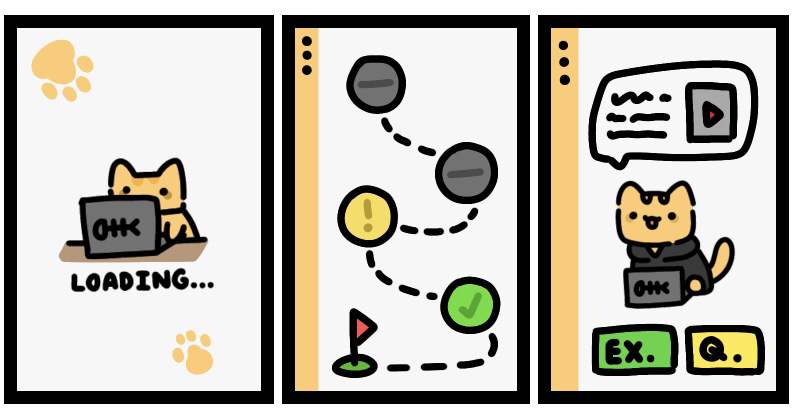
\includegraphics[width = 0.5\textwidth]{UI.png}
    	\caption{Example of the UI}
    	\label{fig:UIExample}
    \end{figure}

\section{Content}
The content that will be used in the game is taken from the class subject EGCI113 - Fundamental Programming. The content will start from simple topics such as type of variable and scanf/printf to more complex topics such as file manipulation. Further topics and details would need to be discussed with our main advisor.

\section{Game Design}
We have thought out the possible types of exercises that will be integrated into the game such as detect the error, code blocking, and fill in the blank (both via typing and drag-\&-drop). We have yet to come to a conclusion on how the lesson part will be presented. We have thought about the lesson being a mixed type where the user will be introduced with the lecture, then they will be led into the exercise part to help them understand and hone their programming skill. We have not yet come up with how the lecture will be presented. Possible integration would be interactive lecture where the mistakes in here will not be counted towards the review calculation and the examples used will be easy for users to understand the basic concept.
	\begin{figure}[!htbp]
		\centering
		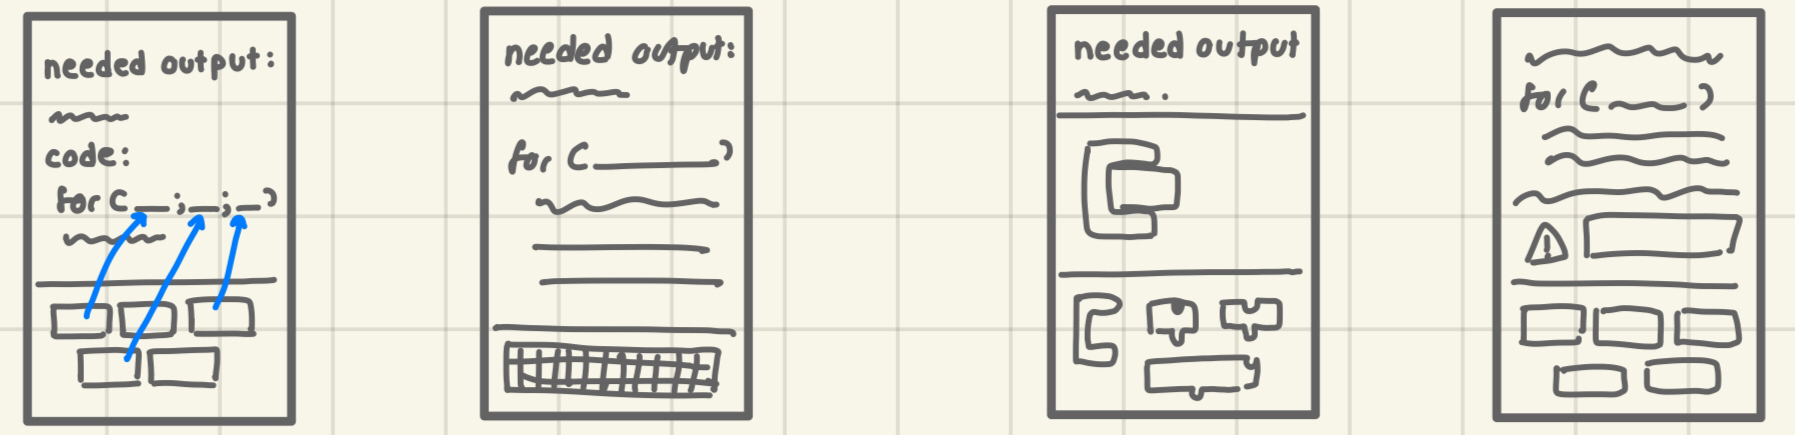
\includegraphics[width = \textwidth]{Exercise.png}
		\caption{Possible Exercises}
		\label{fig:Exercises}
	\end{figure}

\section{Evaluation Method}
Lastly, the evaluation method will possibly be divided into 2 parts: comparison between pure lecture and aided with the application and between our application and other application in the market. We have not yet come up with the sample size or the application that we will be using to compare the result with. Some of the quality that we will use for comparison is engagement. Other possible choices are having pre/post-test and evaluation form.

\chapter{RESULT}
This chapter reports your experiment results or study report proposed in previous chapter. It typically consists of 1) Results in terms of tables or figures and 2) explanation or discussion of your results, study, or key findings.

\section{Results}
\noindent\hspace{2.5em}(Experiment/Results in the forms ofrtables or/and figures)

\section{Discussions}
\noindent\hspace{2.5em}(Interpretation or the meaning of your experiment/results)


\chapter{Conclusion}
This chapter summarizes all of your work. It typically starts with the brief explanation of of what you do such as the objective of your work, design, data, experiment results, key findings, interpretation of your experiment and/or result. The obstacles of your work can also be discussed and finally followed by future work. 

\section{Conclusion}
...
\section{Obstacles}
...
\section{Future Work}
...


\newpage
%---- Bibliography -----
\pagestyle{bibliography}
\bibliography{References} 
\bibliographystyle{abbrvnat}
\label{lastpage}
\newpage
%---- Appendix ----
%\coverAppendix
%\pagestyle{appendix}
%\appendix
%\chapter{TEST APPENDICES}

Node.js is an open source and cross platform JavaScript runtime environment [5]. Node.js allows developers to use JavaScript to write the command line tools and for server-side scripting to produce dynamic web page content before the page publishes to the users’ web browser.

\section{Figure}
Node.js is an asynchronous event-driven JavaScript runtime which is designed to build scalable network applications. It runs with the V8 JavaScript engine outside of the browser. Therefore, Node.js becomes very performant.

\begin{figure}[htbp]
    \centering
\includegraphics[width = 0.5\textwidth]{paragraph.png}
    \caption{Paragraph arrangement}
    \label{fig:paragraph}
\end{figure}

\subsection{Equation}
Node.js is an asynchronous event-driven JavaScript runtime which is designed to build scalable network applications. It runs with the V8 JavaScript
\begin{equation}
E=mc^{2}
\end{equation}
นิยมวางสมการไว้กึ่งกลางหน้ากระดาษ และหมายเลขสมการพิมพ์ชิดขวา

\subsubsection{Coding}
Node.js is an asynchronous event-driven JavaScript runtime which is designed to build scalable network applications. It runs with the V8 JavaScript 

\begin{lstlisting}[language=C]
public static void main(String[] args)
{
	System.out.println(“Hello World”);
}
\end{lstlisting}
\section{Table}
GraphQL is both an API query language and a runtime for executing those queries using your current data. GraphQL allows clients the power to ask for exactly what they need and nothing more, makes it easier to evolve APIs over time, and enables powerful developer tools by providing a clear and intelligible description of the data in your API
\begin{table}[hbt!]
    \caption{ตารางข้อมูลตัวอย่าง}
    \centering
    \begin{tabularx}{\textwidth}{|Y|Y|Y|Y|}
    \hline
       ลำดับที่ & ตัวแปร & ค่าของตัวแปร & ตัวอย่าง  \\
    \hline
        1 & $x$ & 15 & $x=15$\\
    \hline
        2 & $y$ & 30 & $y=30$\\
    \hline
    \end{tabularx}
    \label{tab:my_label}
\end{table}

\subsection{Equation}
Node.js is an asynchronous event-driven JavaScript runtime which is designed to build scalable network applications. It runs with the V8 JavaScript
\begin{equation}
E=mc^{2}
\end{equation}
นิยมวางสมการไว้กึ่งกลางหน้ากระดาษ และหมายเลขสมการพิมพ์ชิดขวา

\subsubsection{Coding}
Node.js is an asynchronous event-driven JavaScript runtime which is designed to build scalable network applications. It runs with the V8 JavaScript 

\begin{lstlisting}[language=C]
public static void main(String[] args)
{
	System.out.println(“Hello World”);
}
\end{lstlisting}
\section{Table}
GraphQL is both an API query language and a runtime for executing those queries using your current data. GraphQL allows clients the power to ask for exactly what they need and nothing more, makes it easier to evolve APIs over time, and enables powerful developer tools by providing a clear and intelligible description of the data in your API
\begin{table}[hbt!]
    \caption{ตารางข้อมูลตัวอย่าง}
    \centering
    \begin{tabularx}{\textwidth}{|Y|Y|Y|Y|}
    \hline
       ลำดับที่ & ตัวแปร & ค่าของตัวแปร & ตัวอย่าง  \\
    \hline
        1 & $x$ & 15 & $x=15$\\
    \hline
        2 & $y$ & 30 & $y=30$\\
    \hline
    \end{tabularx}
    \label{tab:my_label}
\end{table}

\end{document}